\chapter{Robot Configuration}
\label{chap:configuration}

The robot we have used has many sensors and motors alongside accompanying software. We use the hardware to control the robot and to gather information of the robot’s surroundings. 

\begin{figure}
\centering
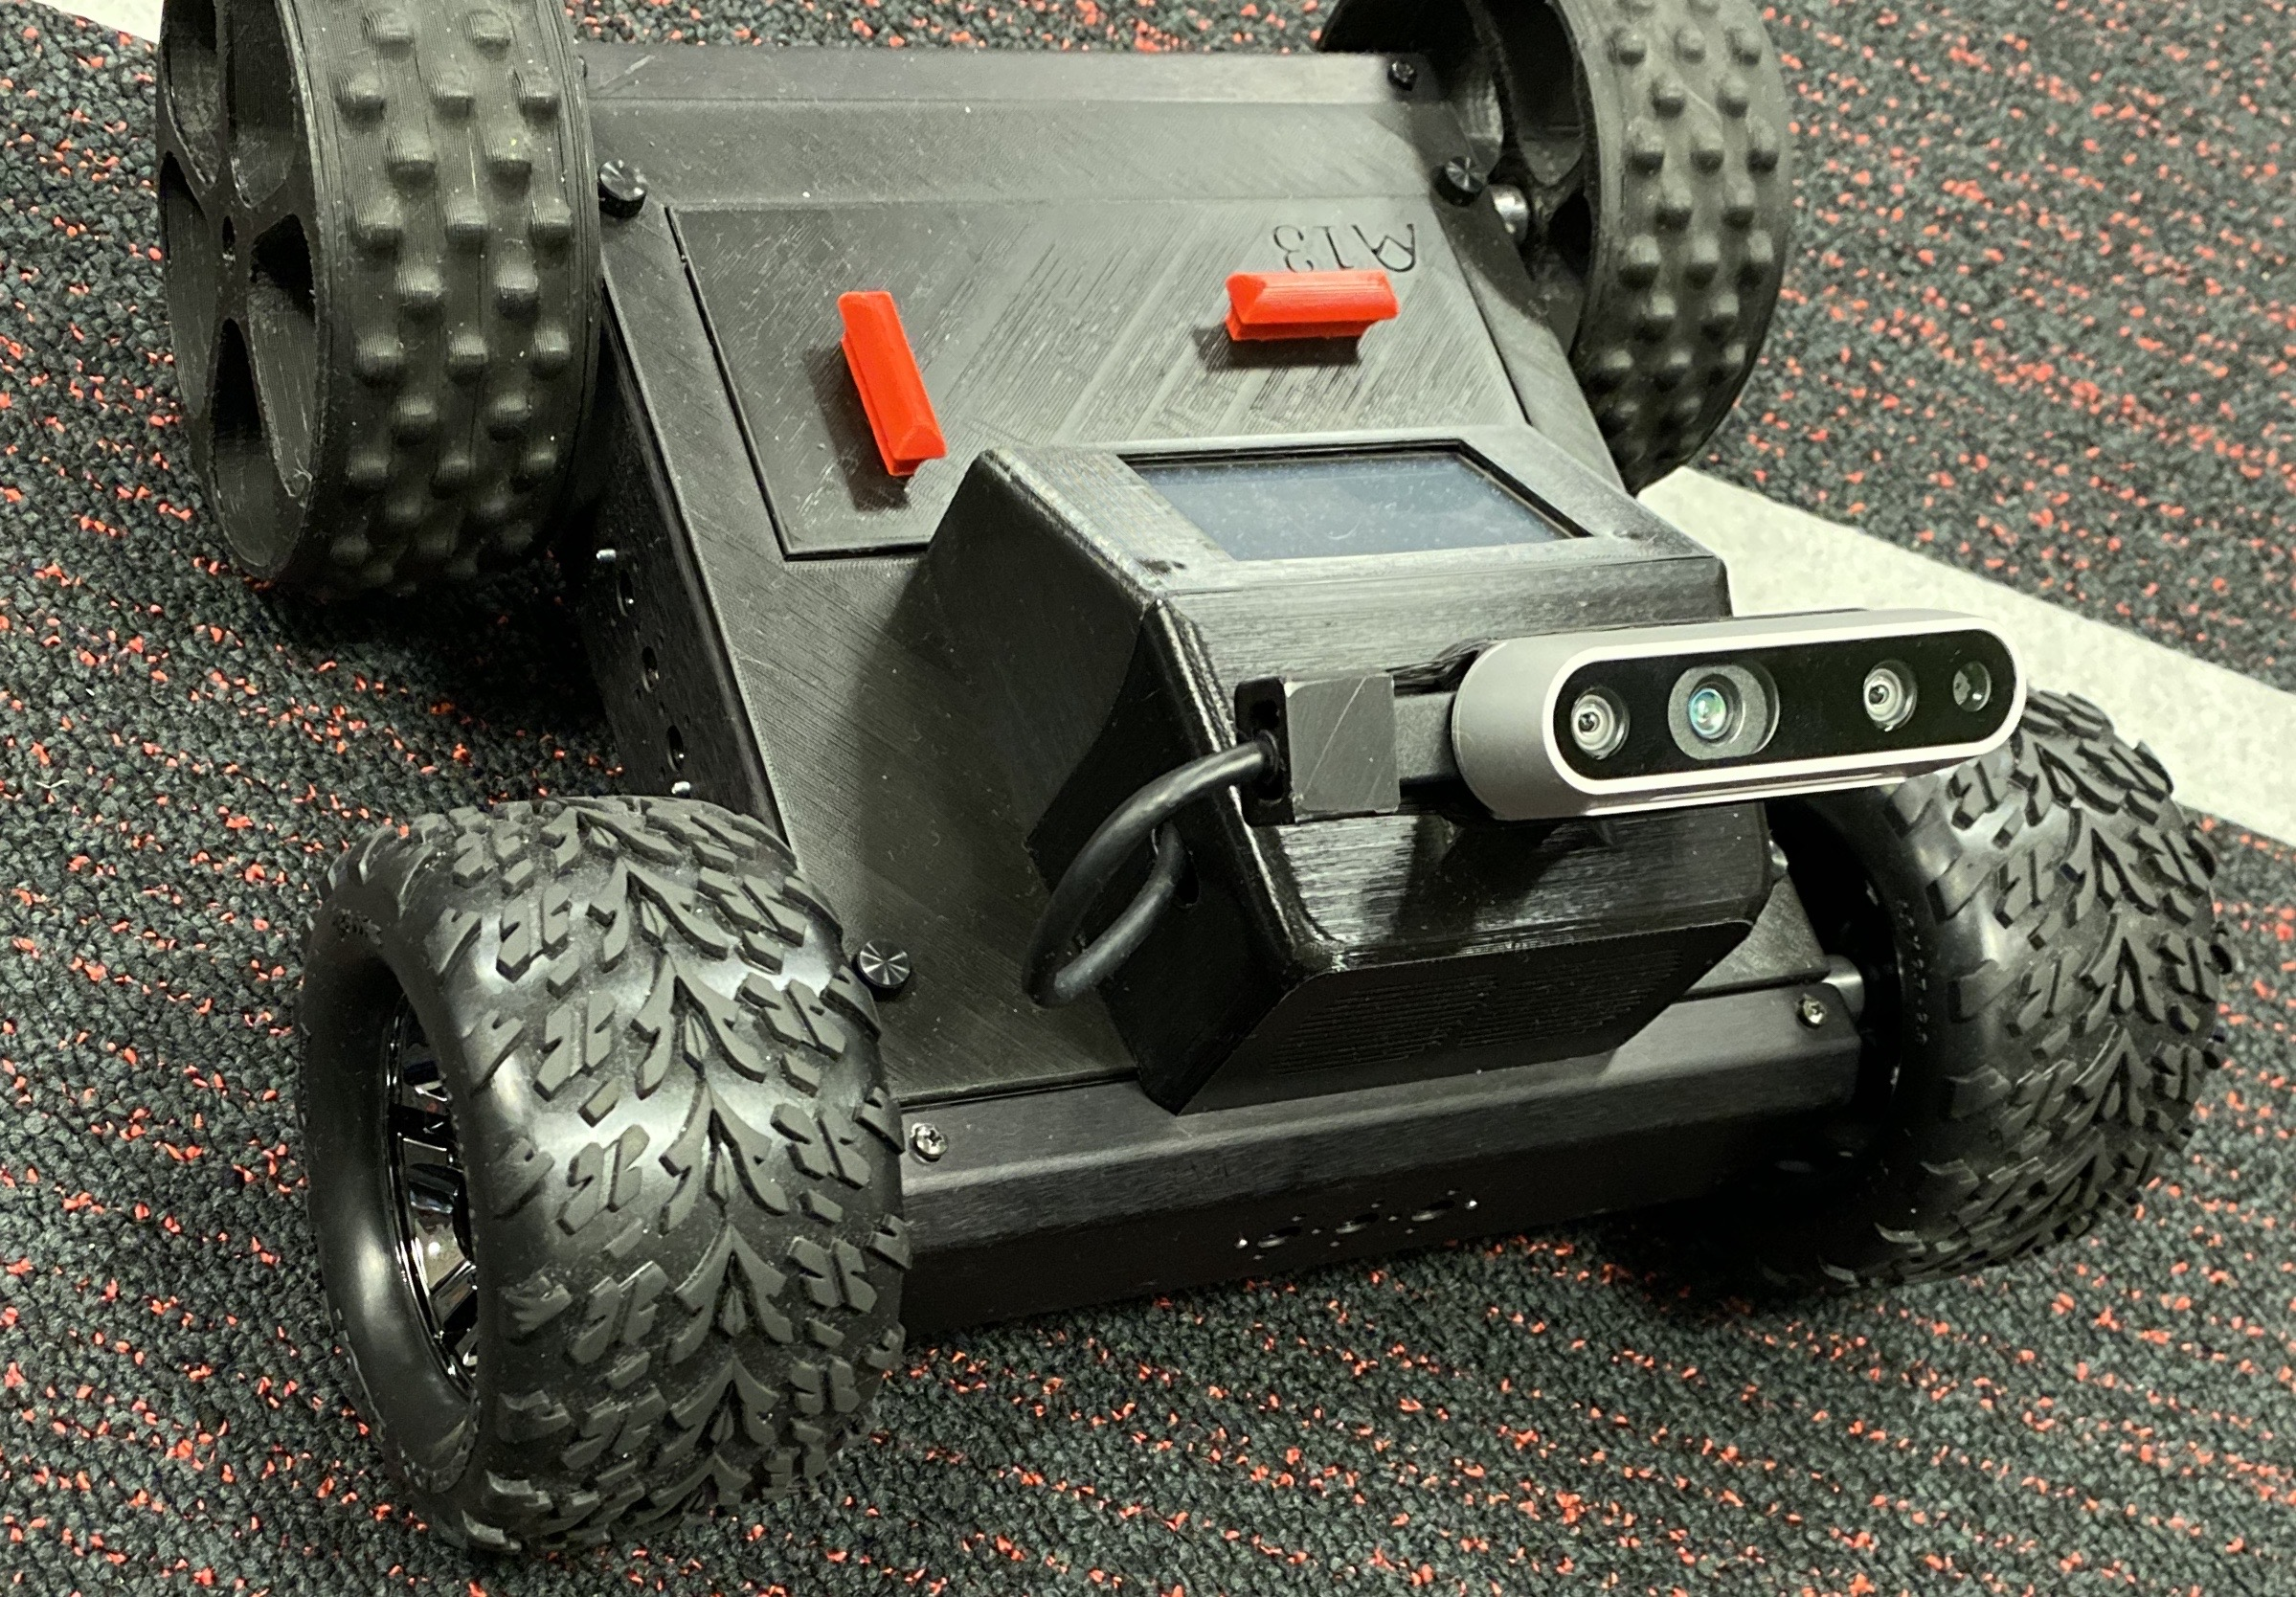
\includegraphics[width=0.5\textwidth]{robot}
\caption{Mobile Robot in This Coursework.}
\label{fig:robot}
\end{figure}

\section{Hardware Components}
\subsection{Motors}
The chassis of the robot is a Lynxmotion Aluminium A4WD1 Rover Kit (w/ Encoders) which contains built in motors and wheels. There are 4 different motors that are default with the rover kit which are 12.0vdc 30:1 gear head motor attached to 4.75” tires and wheels. Each motor can reach up to 7500 RPM and a Motor Driver HAT I2C interface has been installed to the rover kit so that in software we can drive two DC motors at the same time. This allows us to perform forward, forward-left, forward-right, left, right, backward-left and backward-right motion. 

\subsection{Camera}

\begin{figure}
\centering
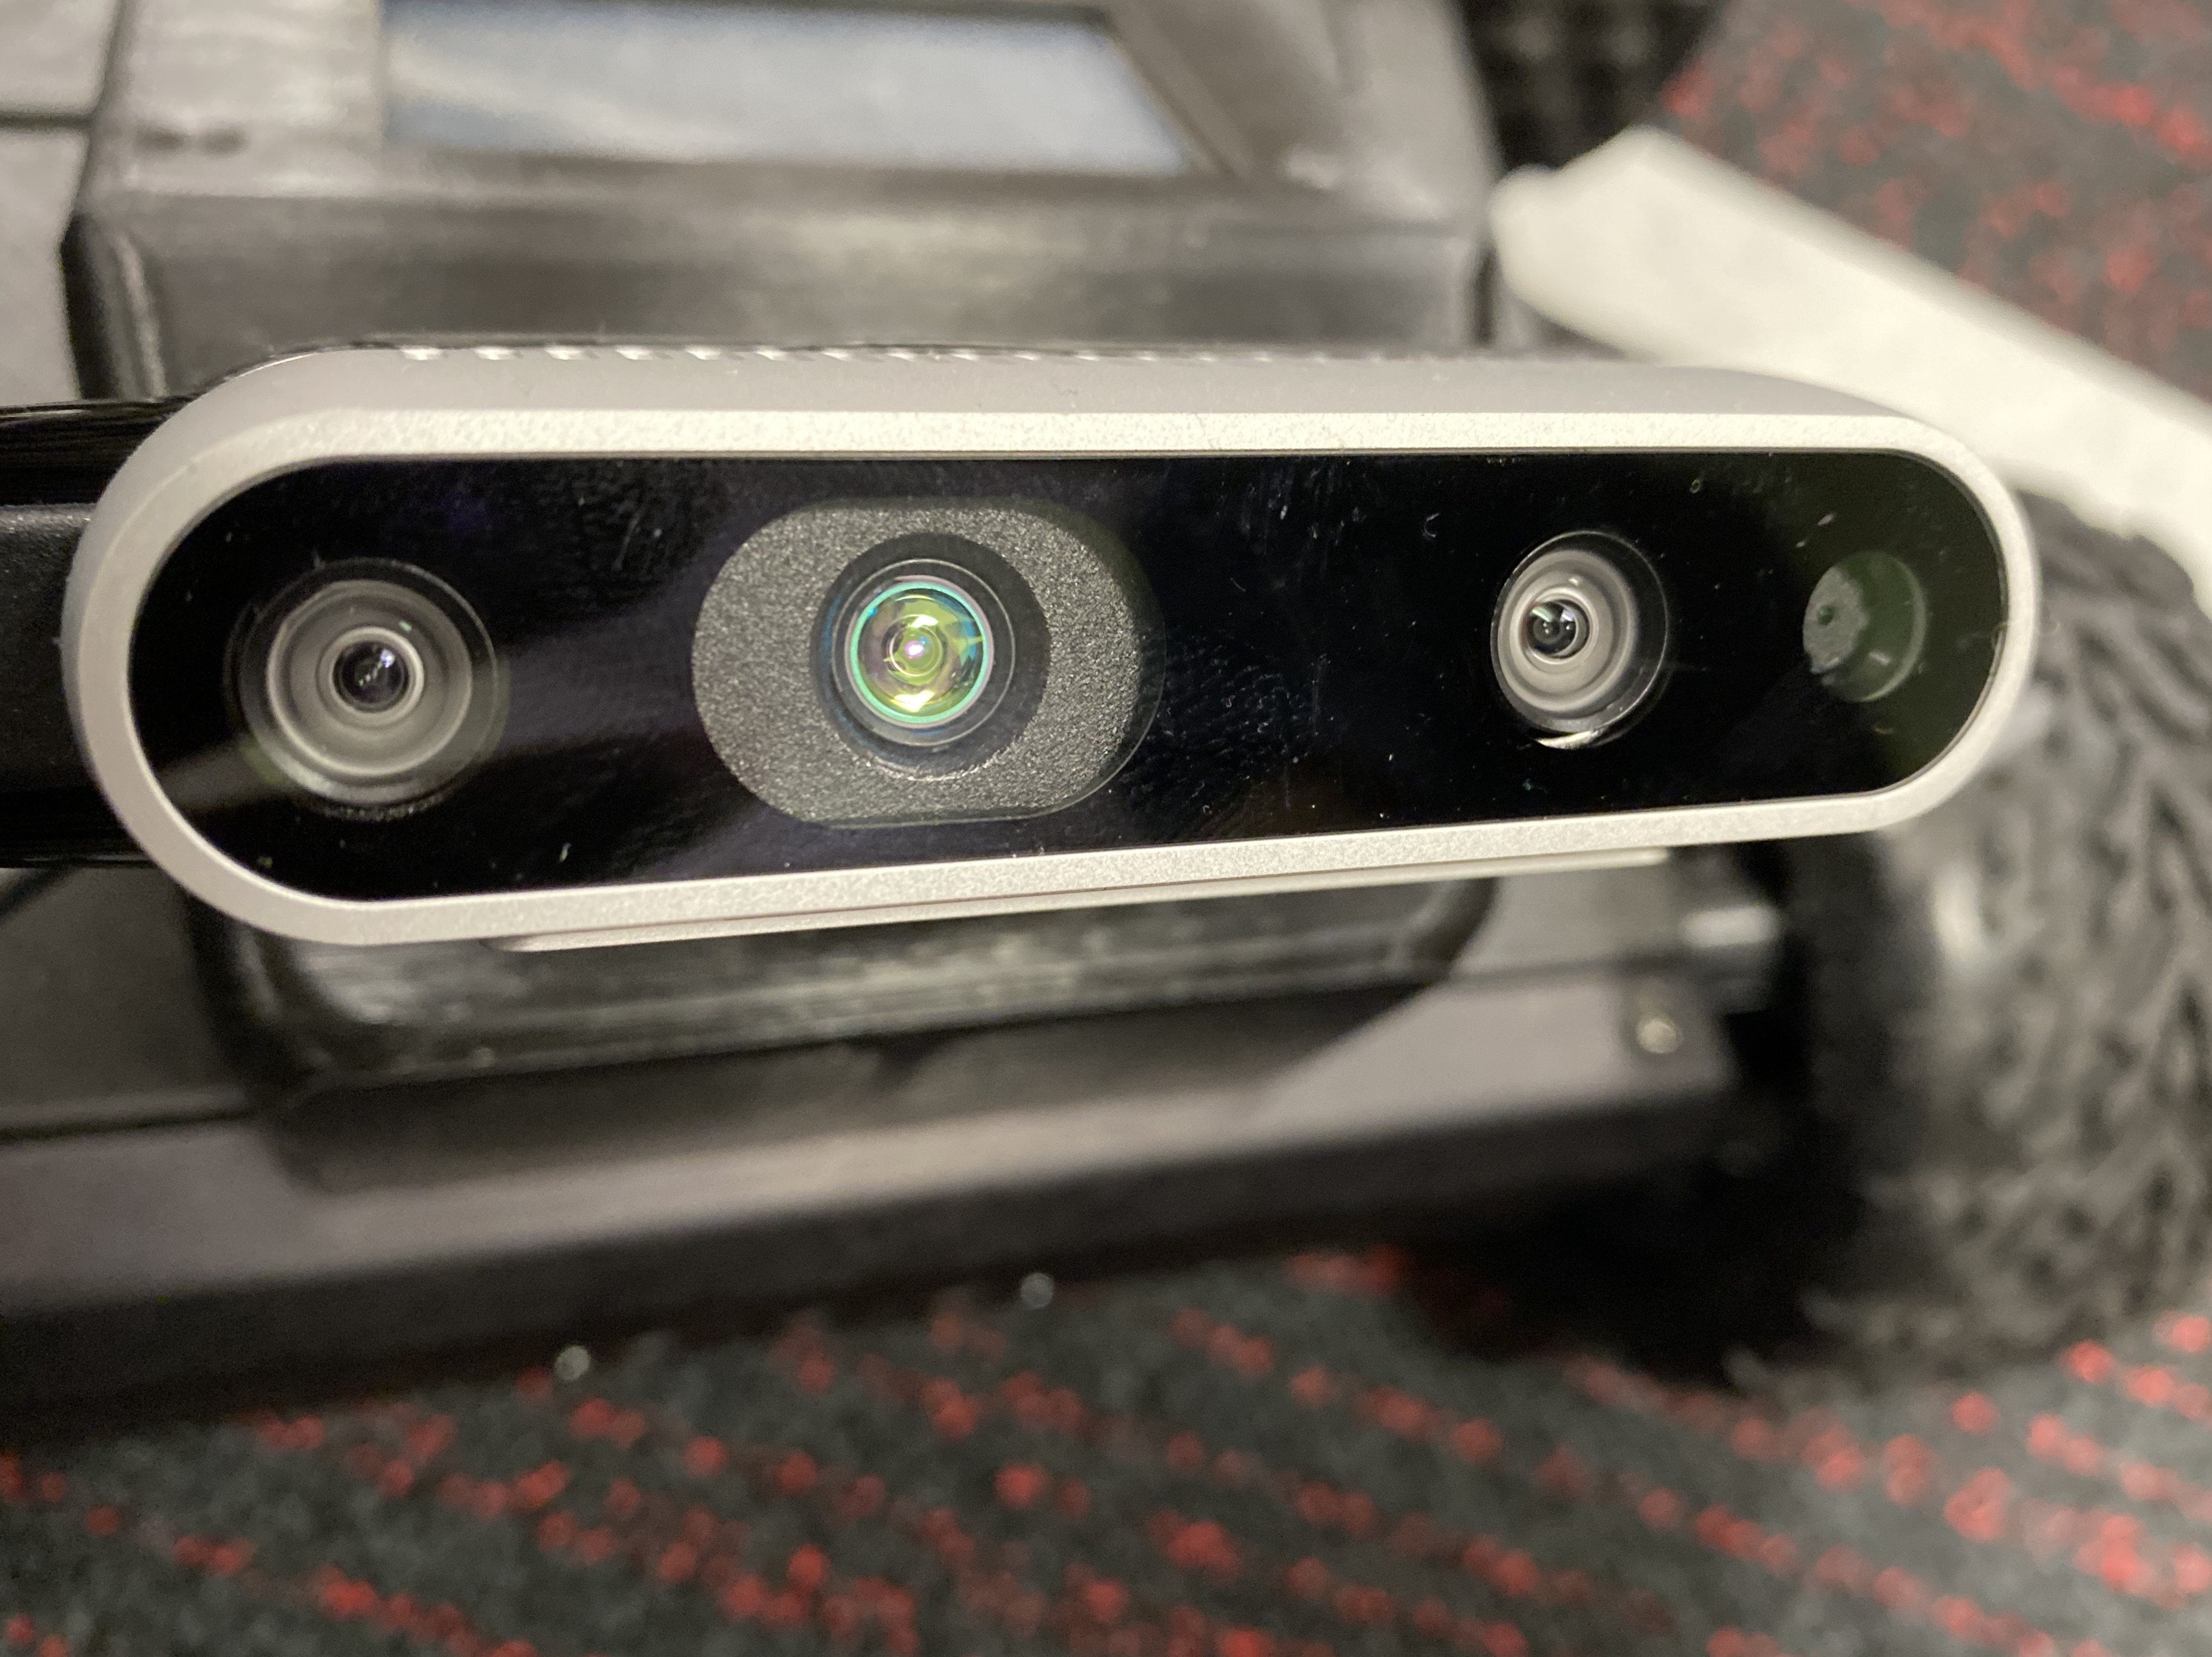
\includegraphics[width=0.5\textwidth]{camera}
\caption{Camera on the Mobile Robot.}
\label{fig:camera}
\end{figure}

The camera that is on the robot is an Intel RealSense Depth Camera D435i which is a colour and depth camera with the addition of an inertial measurement unit (IMU). The IMU refines the camera depth awareness when the camera is moving (i.e. useful for when the robot moves). The depth camera has a depth output resolution and frame rate of 1280x720 active stereo depth resolution up to 90 FPS. The camera RGB feature has a resolution of 1920x1080 with a frame rate of 30 FPS.

There robot has an added Grove IMU 10DOF v2.0 installed at the bottom of the chassis so that we can see the angle of the camera. An issue with IMU is that there can be a drifting affect when stopping so by having two IMU’s it compensates for the drifting for more accurate robot movement. 

\subsection{Wi-Fi Module}
An Intel Dual Band Wireless-AC 8265 Wi-Fi card is installed onto the robot. This allows for remote connectivity and internet access on the robot. 

\subsection{Range Sensor}
There is a range sensor added to the robot which is a VL53L1X Time-of-Flight Distance Sensor Carrier with Voltage Regulator. This sensor is a fast and accurate sensor that ranges up to 4 meters. It uses time of flight of invisible, eye-safe lasers to measure absolute distances independent of lighting conditions and target object characteristics such as colour and shape. 

\subsection{Jetson Nano Developer Kit}
The NVIDIA Jetson Nano Developer kit is a small AI computer that is installed onto the chassis of the robot. This board contains everything needed for us to be able to program the robot and provides access to most of the library functions that were used to control the robot. 

\section{Software Components}
\subsection{Jupyter Notebook}
The software we used to write the code for the robot is called Jupyter Notebook. This is a small cloud IDE that is connected to the robot. For the project we wrote all our Python code in the Jupyter Notebook including running the code, viewing the output of the robot and seeing the information provided by sensors and the camera.

\subsection{Python \& Libraries}
The robot is programmed using Python and the library used to control the robot and its components is called JetBot which is a open-source robot based on NVIDIA Jetson Nano (that is installed on the robot). 

Additionally, built in Python libraries such as Numpy and OpenCV are also used to make programming the robot easier.



